% Conceptual navigation pipeline -- Talos crowd navigation.
% Boxes are functions (not files/nodes); arrows carry signal + update rate.
% Blue = this project's contribution, gray = course-provided / third-party.
% Compile: pdflatex conceptual_pipeline.tex
\documentclass[tikz,border=10pt]{standalone}
\usetikzlibrary{positioning,fit,arrows.meta,backgrounds,calc}

\definecolor{oursblue}{RGB}{31,119,180}
\definecolor{extgray}{RGB}{110,110,110}
\definecolor{goalgreen}{RGB}{34,120,44}

\begin{document}
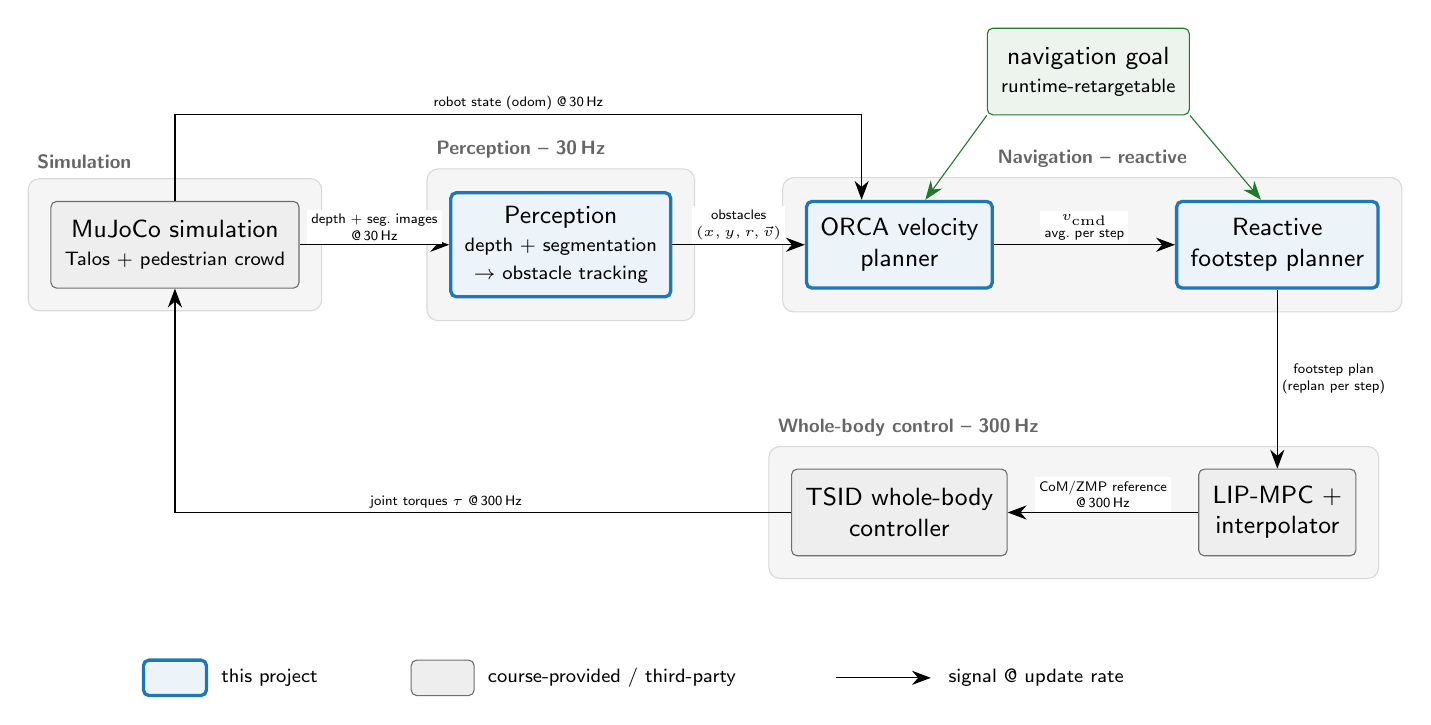
\begin{tikzpicture}[
  font=\sffamily\small,
  >={Stealth[length=2.4mm]},
  block/.style={draw, rounded corners=2pt, align=center, minimum height=11mm,
                inner sep=5pt, fill=white},
  ours/.style={block, draw=oursblue, very thick, fill=oursblue!8},
  ext/.style={block, draw=extgray, fill=extgray!12},
  sig/.style={font=\sffamily\tiny, align=center, fill=white, inner sep=1.5pt},
  band/.style={rounded corners=4pt, inner sep=8pt, fill=black!4, draw=black!15},
  bandlabel/.style={font=\sffamily\scriptsize\bfseries, anchor=south west,
                    text=black!60}
]

% ---------------- blocks ----------------
\node[ext]  (sim)  at (0,0)       {MuJoCo simulation\\[-1pt]\scriptsize Talos + pedestrian crowd};
\node[ours] (perc) at (4.9,0)     {Perception\\[-1pt]\scriptsize depth + segmentation\\[-1pt]\scriptsize $\rightarrow$ obstacle tracking};
\node[ours] (orca) at (9.2,0)     {ORCA velocity\\planner};
\node[ours] (fsp)  at (14.0,0)    {Reactive\\footstep planner};
\node[ext]  (mpc)  at (14.0,-3.4) {LIP-MPC +\\interpolator};
\node[ext]  (tsid) at (9.2,-3.4)  {TSID whole-body\\controller};

% ---------------- bands (background) ----------------
\begin{scope}[on background layer]
  \node[band, fit=(sim)]        (bsim)  {};
  \node[band, fit=(perc)]       (bperc) {};
  \node[band, fit=(orca)(fsp)]  (bnav)  {};
  \node[band, fit=(mpc)(tsid)]  (bwbc)  {};
\end{scope}
\node[bandlabel] at (bsim.north west)  {Simulation};
\node[bandlabel] at (bperc.north west) {Perception -- 30\,Hz};
\node[bandlabel, anchor=south] at (bnav.north) {Navigation -- reactive};
\node[bandlabel] at (bwbc.north west)  {Whole-body control -- 300\,Hz};

% ---------------- main chain ----------------
\draw[->] (sim)  -- node[sig, above]{depth + seg.\ images\\@\,30\,Hz} (perc);
\draw[->] (perc) -- node[sig, above]{obstacles\\$(x,y,r,\vec v)$} (orca);
\draw[->] (orca) -- node[sig, above]{$v_{\mathrm{cmd}}$\\avg.\ per step} (fsp);
\draw[->] (fsp)  -- node[sig, right]{footstep plan\\(replan per step)} (mpc);
\draw[->] (mpc)  -- node[sig, above]{CoM/ZMP reference\\@\,300\,Hz} (tsid);

% ---------------- feedback loops ----------------
\draw[->] (tsid.west) -| node[sig, above, pos=0.28]{joint torques $\tau$ @\,300\,Hz}
          (sim.south);
\draw[->] (sim.north) -- ++(0,1.1)
          -| node[sig, above, pos=0.25]{robot state (odom) @\,30\,Hz} (orca.130);

% ---------------- goal input ----------------
\node[block, draw=goalgreen, fill=goalgreen!8] (goal) at (11.6,2.2)
     {navigation goal\\[-1pt]\scriptsize runtime-retargetable};
\draw[->, goalgreen] (goal.south west) -- (orca.60);
\draw[->, goalgreen] (goal.south east) -- (fsp.110);

% ---------------- legend ----------------
\node[ours, minimum height=4.5mm, minimum width=8mm, inner sep=1pt] (l1) at (0,-5.5) {};
\node[anchor=west, font=\sffamily\scriptsize] at (l1.east) {\,this project};
\node[ext, minimum height=4.5mm, minimum width=8mm, inner sep=1pt] (l2) at (3.4,-5.5) {};
\node[anchor=west, font=\sffamily\scriptsize] at (l2.east) {\,course-provided / third-party};
\draw[->] (8.4,-5.5) -- (9.6,-5.5);
\node[anchor=west, font=\sffamily\scriptsize] at (9.7,-5.5) {signal @ update rate};

\end{tikzpicture}
\end{document}
